\let\negmedspace\undefined
\let\negthickspace\undefined
%\RequirePackage{amsmath}
\documentclass[journal,12pt,twocolumn]{IEEEtran}
%
% \usepackage{setspace}
 \usepackage{gensymb}
  \usepackage[misc]{ifsym}
%\doublespacing
 \usepackage{polynom}
%\singlespacing
%\usepackage{silence}
%Disable all warnings issued by latex starting with "You have..."
%\usepackage{graphicx}
\usepackage{amssymb}
%\usepackage{relsize}
\usepackage[cmex10]{amsmath}
%\usepackage{amsthm}
%\interdisplaylinepenalty=2500
%\savesymbol{iint}
%\usepackage{txfonts}
%\restoresymbol{TXF}{iint}
%\usepackage{wasysym}
\usepackage{amsthm}
%\usepackage{pifont}
%\usepackage{iithtlc}
% \usepackage{mathrsfs}
% \usepackage{txfonts}
 \usepackage{stfloats}
% \usepackage{steinmetz}
 \usepackage{bm}
% \usepackage{cite}
% \usepackage{cases}
% \usepackage{subfig}
%\usepackage{xtab}
\usepackage{longtable}
%\usepackage{multirow}
%\usepackage{algorithm}
%\usepackage{algpseudocode}
\usepackage{enumitem}
 \usepackage{mathtools}
 \usepackage{tikz}
% \usepackage{circuitikz}
% \usepackage{verbatim}
%\usepackage{tfrupee}
\usepackage[breaklinks=true]{hyperref}
%\usepackage{stmaryrd}
%\usepackage{tkz-euclide} % loads  TikZ and tkz-base
%\usetkzobj{all}
\usepackage{listings}
    \usepackage{color}                                            %%
    \usepackage{array}                                            %%
    \usepackage{longtable}                                        %%
    \usepackage{calc}                                             %%
    \usepackage{multirow}                                         %%
    \usepackage{hhline}                                           %%
    \usepackage{ifthen}                                           %%
  %optionally (for landscape tables embedded in another document): %%
    \usepackage{lscape}     
% \usepackage{multicol}
% \usepackage{chngcntr}
%\usepackage{enumerate}
\usepackage{tfrupee}

%\usepackage{wasysym}
%\newcounter{MYtempeqncnt}
\DeclareMathOperator*{\Res}{Res}
\DeclareMathOperator*{\equals}{=}
%\renewcommand{\baselinestretch}{2}
%\renewcommand\thesection{\arabic{section}}
%\renewcommand\thesubsection{\thesection.\arabic{subsection}}
%\renewcommand\thesubsubsection{\thesubsection.\arabic{subsubsection}}

%\renewcommand\thesectiondis{\arabic{section}}
%\renewcommand\thesubsectiondis{\thesectiondis.\arabic{subsection}}
%\renewcommand\thesubsubsectiondis{\thesubsectiondis.\arabic{subsubsection}}

% correct bad hyphenation here
\hyphenation{op-tical net-works semi-conduc-tor}
\def\inputGnumericTable{}                                 %%

\lstset{
%language=C,
frame=single, 
breaklines=true,
columns=fullflexible
}
%\lstset{
%language=tex,
%frame=single, 
%breaklines=true
%}
\begin{document}

%


\newtheorem{theorem}{Theorem}[section]
\newtheorem{problem}{Problem}
\newtheorem{proposition}{Proposition}[section]
\newtheorem{lemma}{Lemma}[section]
\newtheorem{corollary}[theorem]{Corollary}
\newtheorem{example}{Example}[section]
\newtheorem{definition}[problem]{Definition}
%\newtheorem{thm}{Theorem}[section] 
%\newtheorem{defn}[thm]{Definition}
%\newtheorem{algorithm}{Algorithm}[section]
%\newtheorem{cor}{Corollary}
\newcommand{\BEQA}{\begin{eqnarray}}
\newcommand{\EEQA}{\end{eqnarray}}
\newcommand{\define}{\stackrel{\triangle}{=}}
\newcommand*\circled[1]{\tikz[baseline=(char.base)]{
    \node[shape=circle,draw,inner sep=2pt] (char) {#1};}}
\bibliographystyle{IEEEtran}
%\bibliographystyle{ieeetr}
\providecommand{\mbf}{\mathbf}
\providecommand{\pr}[1]{\ensuremath{\Pr\left(#1\right)}}
\providecommand{\qfunc}[1]{\ensuremath{Q\left(#1\right)}}
\providecommand{\sbrak}[1]{\ensuremath{{}\left[#1\right]}}
\providecommand{\lsbrak}[1]{\ensuremath{{}\left[#1\right.}}
\providecommand{\rsbrak}[1]{\ensuremath{{}\left.#1\right]}}
\providecommand{\brak}[1]{\ensuremath{\left(#1\right)}}
\providecommand{\lbrak}[1]{\ensuremath{\left(#1\right.}}
\providecommand{\rbrak}[1]{\ensuremath{\left.#1\right)}}
\providecommand{\cbrak}[1]{\ensuremath{\left\{#1\right\}}}
\providecommand{\lcbrak}[1]{\ensuremath{\left\{#1\right.}}
\providecommand{\rcbrak}[1]{\ensuremath{\left.#1\right\}}}
\theoremstyle{remark}
\newtheorem{rem}{Remark}
\newcommand{\sgn}{\mathop{\mathrm{sgn}}}
\providecommand{\fourier}{\overset{\mathcal{F}}{ \rightleftharpoons}}
%\providecommand{\hilbert}{\overset{\mathcal{H}}{ \rightleftharpoons}}
\providecommand{\system}{\overset{\mathcal{H}}{ \longleftrightarrow}}
	%\newcommand{\solution}[2]{\textbf{Solution:}{#1}}
\newcommand{\solution}{\noindent \textbf{Solution: }}
\newcommand{\cosec}{\,\text{cosec}\,}
\providecommand{\dec}[2]{\ensuremath{\overset{#1}{\underset{#2}{\gtrless}}}}
\newcommand{\myvec}[1]{\ensuremath{\begin{pmatrix}#1\end{pmatrix}}}
\newcommand{\mydet}[1]{\ensuremath{\begin{vmatrix}#1\end{vmatrix}}}
%\numberwithin{equation}{section}
%\numberwithin{figure}{section}
%\numberwithin{table}{section}
%\numberwithin{equation}{subsection}
%\numberwithin{problem}{section}
%\numberwithin{definition}{section}
\makeatletter
\@addtoreset{figure}{problem}
\makeatother
\let\StandardTheFigure\thefigure
\let\vec\mathbf
%\renewcommand{\thefigure}{\theproblem.\arabic{figure}}
\renewcommand{\thefigure}{\theproblem}
%\setlist[enumerate,1]{before=\renewcommand\theequation{\theenumi.\arabic{equation}}
%\counterwithin{equation}{enumi}
%\renewcommand{\theequation}{\arabic{subsection}.\arabic{equation}}
\def\putbox#1#2#3{\makebox[0in][l]{\makebox[#1][l]{}\raisebox{\baselineskip}[0in][0in]{\raisebox{#2}[0in][0in]{#3}}}}
     \def\rightbox#1{\makebox[0in][r]{#1}}
     \def\centbox#1{\makebox[0in]{#1}}
     \def\topbox#1{\raisebox{-\baselineskip}[0in][0in]{#1}}
     \def\midbox#1{\raisebox{-0.5\baselineskip}[0in][0in]{#1}}
\title{
	%\logo{
%Computational Approach to School Geometry
	Assignment
%	}
}
\author{ sumeeth kumar\\AI21BTECH11008
}	
%\title{
%	\logo{Matrix Analysis through Octave}{\begin{center}\includegraphics[scale=.24]{tlc}\end{center}}{}{HAMDSP}
%}
% paper title
% can use linebreaks \\ within to get better formatting as desired
%\title{Matrix Analysis through Octave}
%
%
% author names and IEEE memberships
% note positions of commas and nonbreaking spaces ( ~ ) LaTeX will not break
% a structure at a ~ so this keeps an author's name from being broken across
% two lines.
% use \thanks{} to gain access to the first footnote area
% a separate \thanks must be used for each paragraph as LaTeX2e's \thanks
% was not built to handle multiple paragraphs
%
%\author{<-this % stops a space
%\thanks{}}
%}
% note the % following the last \IEEEmembership and also \thanks - 
% these prevent an unwanted space from occurring between the last author name
% and the end of the author line. i.e., if you had this:
% 
% \author{....lastname \thanks{...} \thanks{...} }
%                     ^------------^------------^----Do not want these spaces!
%
% a space would be appended to the last name and could cause every name on that
% line to be shifted left slightly. This is one of those "LaTeX things". For
% instance, "\textbf{A} \textbf{B}" will typeset as "A B" not "AB". To get
% "AB" then you have to do: "\textbf{A}\textbf{B}"
% \thanks is no different in this regard, so shield the last } of each \thanks
% that ends a line with a % and do not let a space in before the next \thanks.
% Spaces after \IEEEmembership other than the last one are OK (and needed) as
% you are supposed to have spaces between the names. For what it is worth,
% this is a minor point as most people would not even notice if the said evil
% space somehow managed to creep in.
%\WarningFilter{latex}{LaTeX Warning: You have requested, on input line 117, version}
% The paper headers
%\markboth{Journal of \LaTeX\ Class Files,~Vol.~6, No.~1, January~2007}%
%{Shell \MakeLowercase{\textit{et al.}}: Bare Demo of IEEEtran.cls for Journals}
% The only time the second header will appear is for the odd numbered pages
% after the title page when using the twoside option.
% 
% *** Note that you probably will NOT want to include the author's ***
% *** name in the headers of peer review papers.                   ***
% You can use \ifCLASSOPTIONpeerreview for conditional compilation here if
% you desire.
% If you want to put a publisher's ID mark on the page you can do it like
% this:
%\IEEEpubid{0000--0000/00\$00.00~\copyright~2007 IEEE}
% Remember, if you use this you must call \IEEEpubidadjcol in the second
% column for its text to clear the IEEEpubid mark.
% make the title area
\maketitle
\tableofcontents
\bigskip
\renewcommand{\thefigure}{\theenumi}
\renewcommand{\thetable}{\theenumi}
%\renewcommand{\theequation}{\theenumi}
%\begin{abstract}
%%\boldmath
%In this letter, an algorithm for evaluating the exact analytical bit error rate  (BER)  for the piecewise linear (PL) combiner for  multiple relays is presented. Previous results were available only for upto three relays. The algorithm is unique in the sense that  the actual mathematical expressions, that are prohibitively large, need not be explicitly obtained. The diversity gain due to multiple relays is shown through plots of the analytical BER, well supported by simulations. 
%
%\end{abstract}
% IEEEtran.cls defaults to using nonbold math in the Abstract.
% This preserves the distinction between vectors and scalars. However,
% if the journal you are submitting to favors bold math in the abstract,
% then you can use LaTeX's standard command \boldmath at the very start
% of the abstract to achieve this. Many IEEE journals frown on math
% in the abstract anyway.
% Note that keywords are not normally used for peerreview papers.
%\begin{IEEEkeywords}
%Cooperative diversity, decode and forward, piecewise linear
%\end{IEEEkeywords}
% For peer review papers, you can put extra information on the cover
% page as needed:
% \ifCLASSOPTIONpeerreview
% \begin{center} \bfseries EDICS Category: 3-BBND \end{center}
% \fi
%
% For peerreview papers, this IEEEtran command inserts a page break and
% creates the second title. It will be ignored for other modes.
%\IEEEpeerreviewmaketitle
\begin{abstract}
This manual provides solutions to the Assignment of Random Numbers
\end{abstract}
%template ends here
\section{Uniform Random Numbers}
Let $U$ be a uniform random variable between 0 and 1.
\begin{enumerate}[label=\thesection.\arabic*
,ref=\thesection.\theenumi]
\item Generate $10^6$ samples of $U$ using a C program and save into a file called uni.dat .
\\
\solution Download the following files and execute the  C program.
\begin{lstlisting}
wget https://github.com/sumeethkumar12/random-variables/blob/main/1/unidat.c
wget https://github.com/sumeethkumar12/random-variables/blob/main/1/coeffs.h
\end{lstlisting}
Download the above files and execute the following commands
\begin{enumerate}
    \item \$ gcc unidat.c -lm
    \item \$ ./a.out
\end{enumerate}
\item
Load the uni.dat file into python and plot the empirical CDF of $U$ using the samples in uni.dat. The CDF is defined as
\begin{align}
F_{U}(x) = \pr{U \le x}
\end{align}
\\
\solution  The following code plots Fig. \ref{fig:1.2}
\begin{lstlisting}
wget https://github.com/sumeethkumar12/random-variables/blob/main/1/1_2.py
\end{lstlisting}
Download the above files and execute the following commands to produce Fig.\ref{fig:1.2}
\begin{enumerate}
    \item \$ python3 1\_2.py
\end{enumerate}
\begin{figure}[!h]
\centering
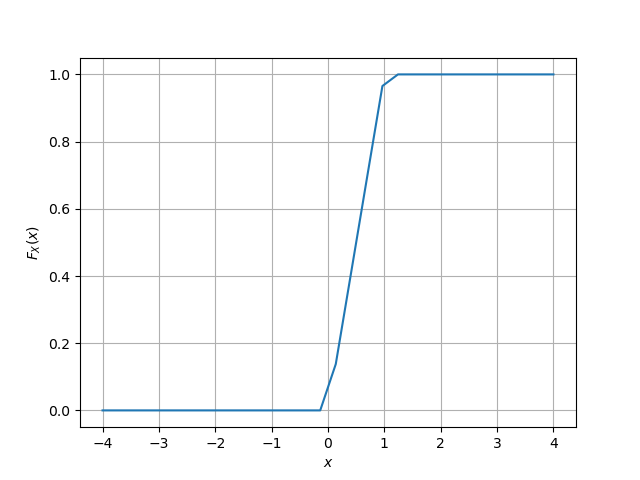
\includegraphics[width=\columnwidth]{1_2cdf.png}
\caption{The CDF of $U$}
\label{fig:1.2}
\end{figure}
%
\item
Find a  theoretical expression for $F_{U}(x)$.\\
\solution Given $U$ is a uniform Random Variable
\begin{align}
p_{U}(x)=1 \text{ for } \\
F_U(x)=\int_{-\infty}^{\infty}p_{U}(x)dx\\
\implies {F_U(x)=x  }
\end{align}
\item
The mean of $U$ is defined as
%
\begin{equation}
E\sbrak{U} = \frac{1}{N}\sum_{i=1}^{N}U_i
\end{equation}
%
and its variance as
%
\begin{equation}
\text{var}\sbrak{U} = E\sbrak{U- E\sbrak{U}}^2 
\end{equation}
Write a C program to  find the mean and variance of $U$. \\
\solution Download the following files and execute the  C program.
\begin{lstlisting}
wget ttps://github.com/sumeethkumar12/random-variables/blob/main/1/1_4.c
wget https://github.com/sumeethkumar12/random-variables/blob/main/1/coeffs.h
\end{lstlisting}
Download the above files and execute the following commands
\begin{enumerate}
    \item \$ gcc 1\_4.c
    \item \$ ./a.out
    \end{enumerate}
\item Verify your result theoretically given that
\end{enumerate}
%
\begin{equation}
E\sbrak{U^k} = \int_{-\infty}^{\infty}x^kdF_{U}(x)
\end{equation}
\solution 
\begin{align}
    \text{var}\sbrak{U} &= E\sbrak{U- E\sbrak{U}}^2\\ 
    \implies \text{var}\sbrak{U} &= E\sbrak{U^2}- E\sbrak{U}^2 \\
    E\sbrak{U}&=\int_{-\infty}^{\infty}xdF_U(x)\\
    E\sbrak{U}&=\int_{0}^{1}x\\
    \implies \boxed{E\sbrak{U}=\frac{1}{2}}\\
    E\sbrak{U^2}&=\int_{-\infty}^{\infty}x^{2}dF_U(x)\\
    E\sbrak{U^2}&=\int_{0}^{1}x^{2}dF_U(x)\\
    \implies E\sbrak{U^2}&=\frac{1}{3}\\
    \implies \boxed{\text{var}\sbrak{U}=\frac{1}{12}=0.0833}
\end{align}
\section{Central Limit Theorem}
%
\begin{enumerate}[label=\thesection.\arabic*
,ref=\thesection.\theenumi]
%
\item
Generate $10^6$ samples of the random variable
%
\begin{equation}
X = \sum_{i=1}^{12}U_i -6
\end{equation}
%
using a C program, where $U_i, i = 1,2,\dots, 12$ are  a set of independent uniform random variables between 0 and 1 and save in a file called gau.dat\\
\solution Download the following files and execute the  C program.
\begin{lstlisting}
wget https://github.com/sumeethkumar12/random-variables/blob/main/2/2_1.c
wget ttps://github.com/sumeethkumar12/random-variables/blob/main/1/coeffs.h
\end{lstlisting}
Download the above files and execute the following commands

\begin{enumerate}
    \item \$ gcc 2\_1.c
    \item \$ ./a.out
    \end{enumerate}
\item
Load gau.dat in python and plot the empirical CDF of $X$ using the samples in gau.dat. What properties does a CDF have?\\
\solution The CDF of $X$ is plotted in Fig. \ref{fig:2.2}\\
using the code below
\begin{lstlisting}
wget https://github.com/sumeethkumar12/random-variables/blob/main/2/2_2.py
\end{lstlisting}
Download the above files and execute the following commands to produce Fig.\ref{fig:2.2}
\begin{enumerate}
    \item \$ python3 2.2.py
\end{enumerate}
\begin{figure}[!h]
\centering
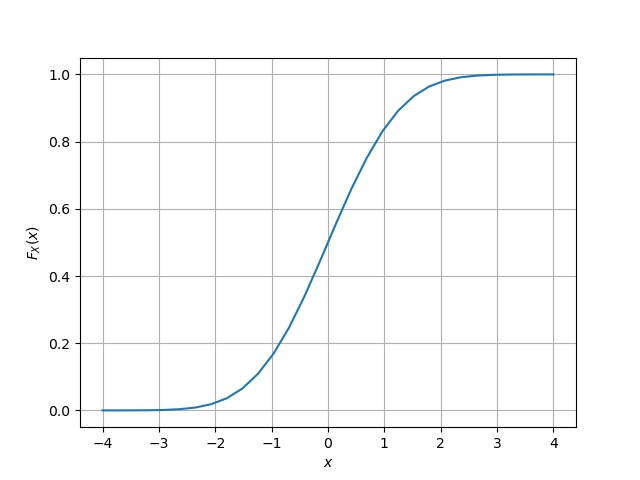
\includegraphics[width=\columnwidth]{2_2gau.png}
\caption{The CDF of $X$}
\label{fig:2.2}
\end{figure}
Some of the properties of CDF 
\begin{enumerate}
    \item $F_X(x)$ is non decreasing function.
    \item Symmetric about one point.
    \item The Q function is defined as,\\
          $Q(X)=Pr(X>x)$
    \item Hence we can use it to calculate  $F_x(x) $,\\
           $F_x(x)=1-Q(x)$
\end{enumerate}
\item
Load gau.dat in python and plot the empirical PDF of $X$ using the samples in gau.dat. The PDF of $X$ is defined as
\begin{align}
p_{X}(x) = \frac{d}{dx}F_{X}(x)
\end{align}
What properties does the PDF have?
\\
\solution The PDF of $X$ is plotted in Fig. \ref{fig:2.3} using the code below
\begin{lstlisting}
wget https://github.com/sumeethkumar12/random-variables/blob/main/2/2_3.py
\end{lstlisting}
Download the above files and execute the following commands to produce Fig.\ref{fig:2.3}
\begin{enumerate}
    \item \$ python3 2\_3.py
\end{enumerate}
\begin{figure}[!h]
\centering
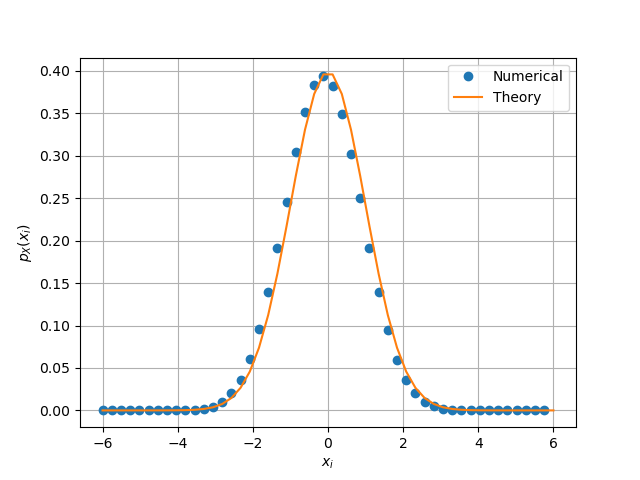
\includegraphics[width=\columnwidth]{2_3pdfgau.png}
\caption{The PDF of $X$}
\label{fig:2.3}
\end{figure}
Some of the properties of the PDF:
\begin{enumerate}
    \item Symmetric about $x=\mu$
    \item decreasing function for $x<\mu$ and increasing for $x>\mu$ and attains maximum at $x=\mu$
    \item Area under the curve is unity.
    
\end{enumerate}
\item Find the mean and variance of $X$ by writing a C program.\\
\solution Download the following files and execute the  C program.
\begin{lstlisting}
wget https://github.com/sumeethkumar12/random-variables/blob/main/2/2_4.c
wget https://github.com/sumeethkumar12/random-variables/blob/main/2/coeffs.h
\end{lstlisting}
Download the above files and execute the following commands
\begin{enumerate}
    \item \$ gcc 2\_4.c
    \item \$ ./a.out
    \end{enumerate}
\item Given that 
\begin{align}
p_{X}(x) = \frac{1}{\sqrt{2\pi}}\exp\brak{-\frac{x^2}{2}}, -\infty < x < \infty,
\end{align}
repeat the above exercise theoretically.
\end{enumerate}
\solution 
\begin{enumerate}
    \item CDF is given by 
    \begin{align}
        F_X(x)&=\int_{-\infty}^{\infty}p_X(x)dx\\
        \boxed{F_X(x)=1}
    \end{align}
    \item Mean is given by
    \begin{align}
        E(x)=\int_{-\infty}^{\infty}xp_X(x)dx\\
        \implies \boxed{E(x)=0}
    \end{align}
    \item Variance is given by
    begin{align*}
    E[X^2] &= \int_{-\infty}  ^{\infty} x^{2} p(x) dx \\[8pt]
    &= x\int_{-\infty} ^{\infty} xp(x) dx - \int_{-\infty} ^{\infty} \left(\int xp(x) dx\right)dx\\[8pt]
    &= \left[-x\frac{1}{\sqrt{2\pi}}e^{\frac{-x^2}{2}}\right]{-\infty} ^{\infty} - \int{-\infty} ^{\infty} -\frac{1}{\sqrt{2\pi}}e^{\frac{-x^2}{2}} dx  \\[8pt]
    &= 0 - (-1)
    &= 1
\end{align*}
$var(x) = E[x^2] - E[x] = 1 - 0 =1$
\end{enumerate}
\section{From Uniform to Other}
\begin{enumerate}[label=\thesection.\arabic*
,ref=\thesection.\theenumi]
%
\item
Generate samples of 
%
\begin{equation}
V = -2\ln\brak{1-U}
\end{equation}
%
and plot its CDF.  \\
\solution Download the following files and execute the  C program.
\begin{lstlisting}
wget https://github.com/sumeethkumar12/random-variables/blob/main/3/3_1.c
wget https://github.com/sumeethkumar12/random-variables/blob/main/3/coeffs.h
\end{lstlisting}
Download the above files and execute the following commands
\begin{enumerate}
    \item \$ gcc 3\_1.c -lm
    \item \$ ./a.out
    \end{enumerate}
The CDF of $V$ is plotted in Fig. \ref{fig:3.1} using the code below
\begin{lstlisting}
wget https://github.com/sumeethkumar12/random-variables/blob/main/3/3_1.py
\end{lstlisting}
Download the above files and execute the following commands to produce Fig.\ref{fig:3.1}
\begin{enumerate}
    \item \$ python3 3\_1.py
\end{enumerate}
\begin{figure}[!h]
\centering
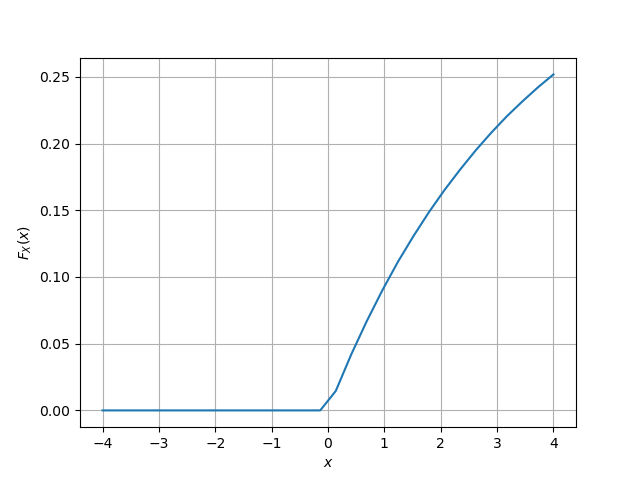
\includegraphics[width=\columnwidth]{3_1.png}\\
\caption{The PDF of $X$}
\label{fig:3.1}
\end{figure}
\item Find a theoretical expression for $F_V(x)$.\\
\solution
If Y = g(X), we know that $F_Y(y) = F_X(g^{-1}(y))$, here 
\begin{align}
V &= -2\ln{(1-U)} \\
1-U &= e^{\frac{-V}{2}}\\
U &= 1 - e^{\frac{-V}{2}} \\ 
F_V(X) &= F_U(1 - e^{\frac{-X}{2}}) 
\end{align}
 when , $0 \le 1 - e^{\frac{-X}{2}} \le 1$
 \begin{align}
 0 &\le e^{\frac{-X}{2}} \le 1 \\
  X &\ge 0 , \text{So,} \\ 
  F_V(X) &= 1 - e^{\frac{-X}{2}}, X \ge 0 \\
  F_V(X) &= 0 , X < 0 
 \end{align}
%\item
%Generate the Rayleigh distribution from Uniform. Verify your result through graphical plots.
 \section{Triangular Distribution}
\begin{enumerate}[label=\thesection.\arabic*
,ref=\thesection.\theenumi]
%
\item Generate
	\begin{align}
		T = U_1+U_2
	\end{align}
\solution Download the below code,
 \begin{lstlisting}
 wget https://github.com/Charanyash/Random-Numbers-/blob/main/codes/Q4/coeffs.h
 wget https://github.com/Charanyash/Random-Numbers-/blob/main/codes/Q4/triangular.c
 \end{lstlisting}
and run the following command,
 \begin{lstlisting}
  cc triangular.c -lm
  ./a.out
 \end{lstlisting}
 You will get required generated random numbers in tri.dat file.		
\item Find the CDF of $T$.\\
 \solution Download the below files,
  \begin{lstlisting}
   wget https://github.com/Charanyash/Random-Numbers-/blob/main/codes/Q4/tri.dat
   wget https://github.com/Charanyash/Random-Numbers-/blob/main/codes/Q4/tri_cdf_plot.py
  \end{lstlisting}
  Run the following command,
  \begin{lstlisting}
   python3 tri_cdf_plot.py
  \end{lstlisting}
  \begin{figure}
   \centering
   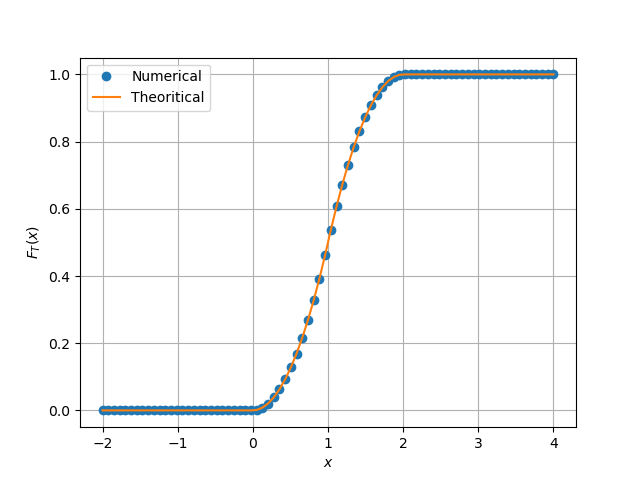
\includegraphics[width=\columnwidth]{Q4/tri_cdf.png}
   \caption{The CDF of $T$}
   \label{fig:tri_cdf}
  \end{figure}
\item Find the PDF of $T$.\\
 \solution Download the below files,
  \begin{lstlisting}
   wget https://github.com/Charanyash/Random-Numbers-/blob/main/codes/Q4/tri.dat
   wget https://github.com/Charanyash/Random-Numbers-/blob/main/codes/Q4/tri_pdf_plot.py
  \end{lstlisting}
  Run the following command,
  \begin{lstlisting}
   python3 tri_pdf_plot.py
  \end{lstlisting}		
 \begin{figure}
  \centering
  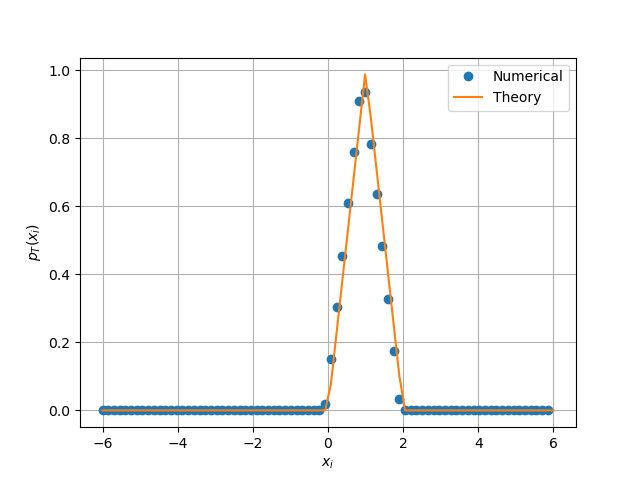
\includegraphics[width=\columnwidth]{Q4/tri_pdf.png}
  \caption{The PDF of $T$}
  \label{fig:tri_pdf}
 \end{figure}
\item Find the theoretical expressions for the PDF and CDF of $T$.\\
  \solution Given that,
   \begin{align}
           T = U1 + U2 \label{eq 4-1} 
   \end{align}
where$ U1, U2 $ are uniform random variables $\in \brak{0,1}$.\\
 \textbf{Calculation of CDF}
The CDF of T is defined as,
   \begin{align}
            F_{T}\brak{t} &= \pr{T \leq t}
   \end{align}
  Now from $\eqref{eq 4-1}$ we can write,
   \begin{align}
           F_{T}\brak{t}  &= \pr{U1 + U2 \leq t}
   \end{align}
 \textbf{Case -1 :} For $ t> 2$.\\
  The $\pr{ U1 + U2 \leq t} = 1$, because for every $ U1 = u1$ and $U2 = u2$, $u1 + u2 <2$,
   \begin{align}
           \implies F_{T}\brak{t} &= 1 
   \end{align}
 \textbf{Case -2 :} For $ t<0$.\\
  The $\pr{ U1 + U2 \leq t} = 0$ because for every $ U1 = u1$ and $U2 = u2$, $u1 + u2 >0$,
   \begin{align}
           \implies F_{T}\brak{t} &= 0 
   \end{align}
 \textbf{Case - 3:} For, $ t \in \brak{0,2} $.\\
  We cannot eliminate the inequality like we did before, so in this case we will operate the inequality by fixing $U1 = x$ where $x\in \brak{0,t} $. So in this case CDF will be,
   \begin{align}
           F_{T}\brak{t}  &= \pr{U1 + U2 \leq t}\\
                          &= \pr{U1 = x,U2 \leq t-x}\\
                          &= \pr{U1 = x}\pr{U2 \leq t-x}  
   \end{align}
 Since U1,U2 are i.i.d.\\
  Now note that $ x$ is a variable and varies in $\brak{0,t}$ , so we have to take integral over x to evaluate the $\pr{U1=x}$ ,
   \begin{align}
           F_{T}\brak{t} &= \int_{0}^{t} f_{U}\brak{x}\pr{U2 \leq t-x} dx\\
                         & =\int_{0}^{t} f_{U}\brak{x}F_{U}\brak{t-x} dx
   \end{align}
\textbf{Case - 1} For $ t \in \brak{0,1} $,we know $f_{U}\brak{x} = 1$ so,
  \begin{align}
          F_{T}\brak{t} &= \int_{0}^{t}1.F_{U}\brak{t-x}dx
  \end{align}
        As, $x<t$ , $ 0<t-x< t<1$ using \eqref{cdf_U},we can write
  \begin{align}
         F_{T}\brak{t} &= \int_{0}^{t}\brak{t-x}dx\\
                       &= \cbrak{ tx - \frac{x^2}{2}}_{0}^{t}\\
                       &= \frac{t^{2}}{2}
  \end{align}
 \textbf{Case -2} For $ t \in \brak{1,2}$ , we know $f_{U}\brak{x} = 0$ at $ x > 1$ ,so the integral solves down to,
  \begin{align}
          F_{T}\brak{t} &= \int_{0}^{1}f_{U}\brak{x}F_{U}\brak{t-x}dx\\
                        &= \int_{0}^{1}1.F_{U}\brak{t-x}dx\\
  \end{align}
   To solve the above integral we will use integration by substitution,
   \begin{align}
            k &= t-x\\
           dk &= -dx\\
           F_{T}\brak{t} &= \int_{t}^{t-1}F_{U}\brak{k}\brak{-dk}\\
                         &= \int_{t-1}^{t}F_{U}\brak{k}dk
   \end{align}
   As $ 1 \leq t \leq 2 , 0 \leq t-1 \leq 1 $ we will break integral at 1 because $ F_{U}\brak{k}$ changes at 1.Using \eqref{cdf_U},
   \begin{align}
           F_{T}\brak{t}  &= \int_{t-1}^{1}F_{U}\brak{k}dk + \int_{1}^{t}F_{U}\brak{k}dk \\
                          &= \int_{t-1}^{1}kdk + \int_{1}^{t}1dk\\
                          &= \cbrak{\frac{k^{2}}{2}}_{t-1}^{1} + t - 1\\
                          &= \frac{1}{2} -\brak{\frac{\brak{t-1}^{2}}{2}} + t - 1\\
                          &= 2t - \frac{t^{2}}{2} - 1
   \end{align}
   Overall we can write the CDF of $F_{T}\brak{x}$ as,
   \begin{align}
           F_{T}\brak{x} &=   \begin{cases}
                                   0                      &,   x <0\\
                                \frac{x^{2}}{2}           &, 0\leq x \leq 1\\
                                2t - \frac{t^{2}}{2} - 1  &, 1 \leq x \leq 2\\
                                   1                      &,   x > 2
                              \end{cases}
    \end{align}      
 \textbf{Calculation of PDF}                
 Now we will find PDF of $T$,\\
 As,
   \begin{align}
           T &= U1 + U2
   \end{align}
  We will use method of convolution to get PDF of $T$ as $ U1$ and $U2$ are i.i.d.
   \begin{align}
          f_{T}\brak{t} &= \int_{-\infty}^{\infty}f_{U1}\brak{x}f_{U2}\brak{t-x}dx
   \end{align}
  Since $ U1,U2$ are of same distribution we can write,
   \begin{align}
           f_{U1}\brak{x} &= f_{U2}\brak{x} = f_{U}\brak{x}\\
           \implies f_{T}\brak{t} &= \int_{-\infty}^{\infty}f_{U}\brak{x}f_{U}\brak{t-x}dx
   \end{align}
 From the PDF of U,we can write
  \begin{align}
          f_{T}\brak{t} &= \int_{0}^{1}f_{U}\brak{x}f_{U}\brak{t-x}dx\\
                        &= \int_{0}^{1}1.f_{U}\brak{t-x}dx\\
  \end{align}
  we will solve the above integral using substitution.
  \begin{align}
            z &= t-x \\
           dz &= -dx \\
          \implies f_{T}\brak{t} &= \int_{t}^{t-1}f_{U}\brak{z}\brak{-dz}\\
                                 &= \int_{t-1}^{t}f_{U}\brak{z}dz
  \end{align}
 \textbf{Case -1} For $ t<0 $ as $ z <t $,the PDF $ f_{U}\brak{z} = 0 $. So,
  \begin{align}
          f_{T}\brak{t} &= 0
  \end{align}
 \textbf{Case -2} For $ 0 \leq t \leq 1$, we will break the integral at $z = 0$, since $f_{U}\brak{z}$ changes at 0.
  \begin{align}
          f_{T}\brak{t} &= \int_{t-1}^{0}f_{U}\brak{z}dz + \int_{0}^{t}f_{U}\brak{z}dz\\
                        &= 0 + \int_{0}^{t}1dz \\
                        &= t
  \end{align}
 \textbf{Case-3} Similarly for $ 1 \leq t \leq 2$, we will break the integral at $ z = 1 $,
  \begin{align}
          f_{T}\brak{t} &= \int_{t-1}^{1}f_{U}\brak{z}dz + \int_{1}^{t}f_{U}\brak{z}\\
                        &= \int_{t-1}^{1}1.dz + 0\\
                        &=  2 - t
  \end{align}
   \textbf{Case-4} For $ t>2$,as $ z > t - 1  > 1$,the PDF $f_{U}\brak{z} = 0 $. So,
   \begin{align}
           f_{T}\brak{z} &= 0
   \end{align}
  Overall, the PDF of T will be,
   \begin{align}
           f_{T}\brak{x} &=  \begin{cases}
                                     0     &, x <0 \\
                                     x     &, 0 \leq x \leq 1\\
                                    2-x    &, 1 \leq x \leq 2 \\
                                     0     &, x > 2
                             \end{cases}
   \end{align}
\item Verify your results through a plot.\\
  \solution This is already done in \ref{fig:tri_cdf} ,\ref{fig:tri_pdf}.
\end{enumerate}
\section{Maximum Likelihood}
\begin{enumerate}[label=\thesection.\arabic*
,ref=\thesection.\theenumi]
\item Generate equiprobable $X \in \cbrak{1,-1}$.\\	
  \solution The generating X or bernoulie random variable $ \brak{X}$ is done by using uni.dat file. Download the below files
    \begin{lstlisting}
         wget https://github.com/Charanyash/Random-Numbers-/blob/main/codes/Q5/coeffs.h
	 wget https://github.com/Charanyash/Random-Numbers-/blob/main/codes/Q5/bernoulie.c
    \end{lstlisting}
  Run the following command
    \begin{lstlisting}
	  cc bernoulie.c -lm
	  ./a.out 
    \end{lstlisting} 
\item Generate
\begin{equation}
Y = AX+N,
\end{equation}
	where $A = 5$ dB,  and $N \sim \gauss{0}{1}$.\\
  \solution To generate distribution of Y random variable we will need previously generated bernoulie distribution and gaussian distribution.Download the below files
    \begin{lstlisting}
     wget  https://github.com/Charanyash/Random-Numbers-/blob/main/codes/Q5/coeffs.h
     wget https://github.com/Charanyash/Random-Numbers-/blob/main/codes/Q5/Y.c
    \end{lstlisting}
   Then run the following command,
    \begin{lstlisting}
     cc Y.c -lm
     ./a.out
    \end{lstlisting}
\item Plot $Y$ using a scatter plot.\\
 \solution Download the below files
    \begin{lstlisting}
      wget https://github.com/Charanyash/Random-Numbers-/blob/main/codes/Q5/Y.py
      wget https://github.com/Charanyash/Random-Numbers-/blob/main/codes/Q5/Y.dat
    \end{lstlisting}
   Then run the following command,
    \begin{lstlisting}
      python3 Y.py
    \end{lstlisting}		
\item Guess how to estimate $X$ from $Y$.
	\solution When $ Y > 0 $, we can more probably say that $X = 1$ as $X$ can take values from $\sbrak{-1,1}$.As $A$ increases the signal contribution will increase compared to noise.The scatter plot will not be intermixed as $A$ increases. So in this case, the scatter plot of $Y$ is seperated with decision boundary as $0$. So we can more probably say that,
	  \begin{align}
		  X &= \begin{cases}
			  1 &, Y>0\\
			 -1 &, Y<0 
		       \end{cases}
          \end{align}		       
\item
\label{ml-ch4_sim}
Find
\begin{equation}
	P_{e|0} = \pr{\hat{X} = -1|X=1}
\end{equation}
and
\begin{equation}
	P_{e|1} = \pr{\hat{X} = 1|X=-1}
\end{equation}
%
\solution The $\hat{X}$ is defined as,
  \begin{align}
      \hat{X} &= \begin{cases}
	             1  &, Y > 0\\
		         0  &, Y\leq 0
		         \end{cases}
  \end{align}
 The error probability, when the actual signal is $X=1$ but transmitted as $\hat{X} = -1$ is,
  \begin{align}
	  P_{e|0} &= \pr{\hat{X} = -1|X=1}\\
	          &= \pr{ Y \leq 0| X= 1}\\
		  &= \pr{AX + N \leq 0 | X=1}\\
		  &= \pr{ A + N \leq 0}\\
		  &= \pr{N \leq -A}\\
		  &= F_{N}\brak{-A}\\
		  &= 0 \label{eq-5.5.1}
  \end{align}
 And for the case when actual signal is $X=-1$ but transmitted as $\hat{X} = 1$ the error probability will be,
  \begin{align}
	  P_{e|1} &= \pr{\hat{X} = 1|X=-1}\\
                  &= \pr{ Y > 0| X=-1}\\
                  &= \pr{AX + N > 0 | X=1}\\
                  &= \pr{ N-A > 0}\\
                  &= \pr{N > A}\\
		  &= 1 - F_{N}\brak{A}\\
		  &= F_{N}\brak{-A}\\
		  &= 0 \label{eq-5.5.2}
  \end{align}
The above calculations are coded in below python file,
  \begin{lstlisting}
    wget  https://github.com/Charanyash/Random-Numbers-/tree/main/codes/Q5/5.5.py
  \end{lstlisting}
  Run the following command
  \begin{lstlisting}
   python3 5.5.py
  \end{lstlisting}
\item Find $P_e$ assuming that $X$ has equiprobable symbols.
%
\item
Verify by plotting  the theoretical $P_e$ with respect to $A$ from 0 to 10 dB.
%
\item Now, consider a threshold $\delta$  while estimating $X$ from $Y$. Find the value of $\delta$ that maximizes the theoretical $P_e$.
\item Repeat the above exercise when
	\begin{align}
		p_{X}(0) = p
	\end{align}
\item Repeat the above exercise using the MAP criterion.
		\end{enumerate}
\section{Gaussian to Other}
\begin{enumerate}[label=\thesection.\arabic*
,ref=\thesection.\theenumi]
\item
Let $X_1 \sim  \gauss{0}{1}$ and $X_2 \sim  \gauss{0}{1}$. Plot the CDF and PDF of
%
\begin{equation}
V = X_1^2 + X_2^2
\end{equation}
%
%
%
\item
If
%
\begin{equation}
F_{V}(x) =
\begin{cases}
1 - e^{-\alpha x} & x \geq 0 \\
0 & x < 0,
\end{cases}
\end{equation}
%
find $\alpha$.
%
\item
\label{ch3_raleigh_sim}
Plot the CDF and PDf of
%
\begin{equation}
A = \sqrt{V}
\end{equation}
%
\end{enumerate}
\section{Conditional Probability}
\begin{enumerate}[label=\thesection.\arabic*
,ref=\thesection.\theenumi]
\item
\label{ch4_sim}
Plot
\begin{equation}
P_e = \pr{\hat{X} = -1|X=1}
\end{equation}
%
for
\begin{equation}
Y = AX+N,
\end{equation}
where $A$ is Raleigh with $E\sbrak{A^2} = \gamma, N \sim \gauss{0}{1}, X \in \brak{-1,1}$ for $0 \le \gamma \le 10$ dB.
%
\item
Assuming that $N$ is a constant, find an expression for $P_e$.  Call this $P_e(N)$
%
\item
%
\label{ch4_anal}
For a function $g$,
\begin{equation}
E\sbrak{g(X)} = \int_{-\infty}^{\infty}g(x)p_{X}(x)\, dx
\end{equation}
%
Find $P_e = E\sbrak{P_e(N)}$.
%
\item
Plot $P_e$ in problems \ref{ch4_sim} and \ref{ch4_anal} on the same graph w.r.t $\gamma$.  Comment.
		\end{enumerate}
\section{Two Dimensions}
Let
\begin{equation}
\mbf{y} = A\mbf{x} + \mbf{n},
\end{equation}
where
\begin{align}
x &\in \brak{\mbf{s}_0,\mbf{s}_1},
\mbf{s}_0 =
\begin{pmatrix}
1
\\
0
\end{pmatrix},
\mbf{s}_1 =
\begin{pmatrix}
0
\\
1
\end{pmatrix}
\\
\mbf{n} &=
\begin{pmatrix}
n_1
\\
n_2
\end{pmatrix},
n_1,n_2 \sim \gauss{0}{1}.
\end{align}
%
\begin{enumerate}[label=\thesection.\arabic*
,ref=\thesection.\theenumi]
%%
\item
\label{ch5_fsk}
Plot
%
\begin{equation}
\mbf{y}|\mbf{s}_0 \text{ and } \mbf{y}|\mbf{s}_1
\end{equation}
%
on the same graph using a scatter plot.
%
\item
For the above problem, find a decision rule for detecting the symbols $\mbf{s}_0 $ and $\mbf{s}_1$.
%
\item
Plot
\begin{equation}
P_e = \pr{\hat{\mbf{x}} = \mbf{s}_1|\mbf{x} = \mbf{s}_0}
\end{equation}
with respect to the SNR from 0 to 10 dB.
%
\item
Obtain an expression for $P_e$. Verify this by comparing the theory and simulation plots on the same graph.
%
		\end{enumerate}
\end{enumerate}
\end{document}
